
%% Dokumenteinstellungen %%%%%%%%%%%%%%%%%%%%%%%%%%%%%%%%%%%%
\documentclass[a4paper,oneside,12pt,ngerman]{scrartcl}

%% Deutsche Anpassungen %%%%%%%%%%%%%%%%%%%%%%%%%%%%%%%%%%%%%
\usepackage[ngerman]{babel}
\usepackage[T1]{fontenc}
\usepackage[ansinew]{inputenc}
\usepackage{lmodern} %Type1-Schriftart f�r nicht-englische Texte
\usepackage{booktabs}	% sch�nere tabellen

%% Packages f�r Grafiken & Abbildungen %%%%%%%%%%%%%%%%%%%%%%
\usepackage{graphicx} %%Zum Laden von Grafiken
%\usepackage{subfig} %%Teilabbildungen in einer Abbildung
%\usepackage{tikz} %%Vektorgrafiken aus LaTeX heraus erstellen


%% Packages f�r Formeln %%%%%%%%%%%%%%%%%%%%%%%%%%%%%%%%%%%%%
\usepackage{amsmath}
\usepackage{amsthm}
\usepackage{amsfonts}


%% Andere Packages %%%%%%%%%%%%%%%%%%%%%%%%%%%%%%%%%%%%%%%%%%
%\usepackage{a4wide} %%Kleinere Seitenr�nder = mehr Text pro Zeile.
\usepackage{fancyhdr} %%Fancy Kopf- und Fu�zeilen
%\usepackage{longtable} %%F�r Tabellen, die eine Seite �berschreiten
\usepackage{lastpage}
\usepackage[raggedright]{subfigure}
\usepackage[final]{pdfpages}
\includepdfset{pages=-,noautoscale}

%%%%%%%%%%%%%%%%%%%%%%%%%%%%%%%%%%%%%%%%%%%%%%%%%%%%%%%%%%%%%
%% TODO
%%%%%%%%%%%%%%%%%%%%%%%%%%%%%%%%%%%%%%%%%%%%%%%%%%%%%%%%%%%%%
% 
% 
%%%%%%%%%%%%%%%%%%%%%%%%%%%%%%%%%%%%%%%%%%%%%%%%%%%%%%%%%%%%%



%%%%%%%%%%%%%%%%%%%%%%%%%%%%%%%%%%%%%%%%%%%%%%%%%%%%%%%%%%%%%
%% Optionen / Modifikationen
%%%%%%%%%%%%%%%%%%%%%%%%%%%%%%%%%%%%%%%%%%%%%%%%%%%%%%%%%%%%%
%%%%%%%%%%%%%%%%%%%%%%%%%%%%%%%%%%%%%%%%%%%%%%%%%%%%%%%%%%%%%
%%                                                         %%
%%                     EINSTELLUNGEN                       %%
%%                                                         %%
%%%%%%%%%%%%%%%%%%%%%%%%%%%%%%%%%%%%%%%%%%%%%%%%%%%%%%%%%%%%%

%%%%%%%%%%%%%%%%%%%%%%%%%%%%%%%%%%%%%%%%%%%%%%%%%%%%%%%%%%%%%
%% HYPER REF
%%%%%%%%%%%%%%%%%%%%%%%%%%%%%%%%%%%%%%%%%%%%%%%%%%%%%%%%%%%%%
\usepackage[
hyperindex=true,
colorlinks=true,
linkcolor=black,
citecolor=black,
filecolor=black,
menucolor=black,
urlcolor=cyan,
breaklinks=true,
bookmarks=true,
bookmarksopen=false,
bookmarksnumbered=false,
pdfhighlight=/O,
]{hyperref}

%%%%%%%%%%%%%%%%%%%%%%%%%%%%%%%%%%%%%%%%%%%%%%%%%%%%%%%%%%%%%
%% FANCY HEADERS
%%%%%%%%%%%%%%%%%%%%%%%%%%%%%%%%%%%%%%%%%%%%%%%%%%%%%%%%%%%%%
% --- Kopf- und Fusszeilen - {} = rechts (gerade), [] = links (ungerade)
% letzte seite: \pageref{LastPage}
% doppelseitig:
%\lhead{Elektronik: \textbf{Oszilatorschaltungen}}	\chead{}		\rhead{Cyril Stoller und Hannes Stauffer}
%\lfoot{\today}	\cfoot{}		\rfoot{Seite \thepage\ von \pageref{LastPage}}

% einseitig:
%\lhead{\rightmark}			\chead{}					\rhead{}
%\lfoot{\leftmark}			\cfoot{}					\rfoot{Seite \thepage\ von \pageref{\LastPage}}

%\setlength{\headrulewidth}{0.4pt}
%\setlength{\footrulewidth}{0.4pt}


% Formeln r�misch nummerieren
\renewcommand{\theequation}{\Roman{equation}} 

% "Formel" statt "Gleichung"
\def\equationname{Formel}

%%%%%%%%%%%%%%%%%%%%%%%%%%%%%%%%%%%%%%%%%%%%%%%%%%%%%%%%%%%%%
%% DOKUMENT
%%%%%%%%%%%%%%%%%%%%%%%%%%%%%%%%%%%%%%%%%%%%%%%%%%%%%%%%%%%%%
\begin{document}

\title{Projektarbeit: High Power RGB-LED}
\date{\today}
\author{Cyril Stoller, Marcel B�rtschi}
\maketitle

%% Inhaltsverzeichnis %%%%%%%%%%%%%%%%%%%%%%%%%%%%%%%%%%%%%%%
\tableofcontents %Inhaltsverzeichnis

\vfill

\listoffigures

%\pagestyle{fancy} %%Ab hier die Kopf-/Fusszeilen: headings / fancy / ...

\newpage

\begin{abstract}
	
\begin{center}	
\textbf{Abstract}
\vspace{0.3cm}

	Um unsere Kentnisse in VHDL und im Entwerfen von elektronischen Schaltungen zu vertiefen, haben wir ein Projekt erarbeitet, in welchem wir beides gleichermassen �ben k�nnen. Dabei ist das Projekt 40 Watt high power LED entstanden. 
\end{center}
	
\end{abstract}

\vspace{2cm}


%%%%%%%%%%%%%%%%%%%%%%%%%%%%%%%%%%%%%%%%%%%%%%%%%%%%%%%%%%%%%
%%                                                         %%
%%         Kapitel / Hauptteil des Dokumentes              %%
%%                                                         %%
%%%%%%%%%%%%%%%%%%%%%%%%%%%%%%%%%%%%%%%%%%%%%%%%%%%%%%%%%%%%%



\section{Ziel}
\begin{quote}
Es gibt nichts Praktischeres als eine gute Theorie.

Immanuel Kant (1724 - 1804), deutscher Philosoph
\end{quote}
Um trotzdem mal selbst Hand anzulegen, ist ein Projekt zu erarbeiten, dass einen digitalen und einen analogen Teil enth�lt. Der zeitliche Rahmen ist auf ein halbes Semester begrenzt. 
Der digitale Teil soll mit einem Spartan 3E Board in VHDL realisiert werden. F�r den analogen Teil sind keine Vorgaben vorhanden.

\section{Einleitung}
Wir haben uns daf�r entschieden, eine RGB-LED im HSV-Farbraum\footnote{Siehe \url{https://de.wikipedia.org/wiki/HSV-Farbraum}} anzusteuern.

Dazu sollen mit dem Dreh-Encoder und vier Tastern die drei Werte \emph{Hue} (Farbwert), \emph{Value} (Dunkelstufe) und \emph{Saturation} (S�ttigung) ver�ndert werden k�nnen.

\begin{figure}[ht]
	\centering
		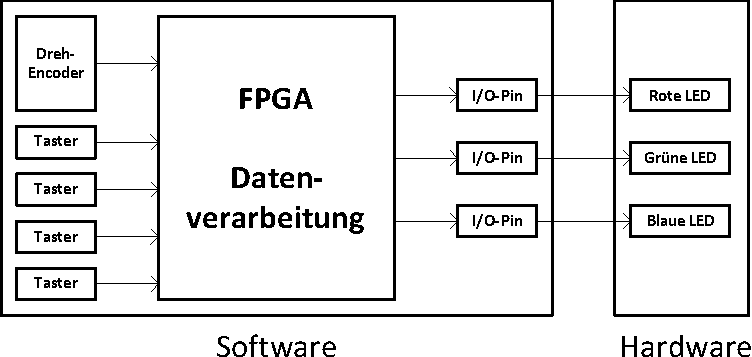
\includegraphics[width=0.70\textwidth]{images/Blockschaltbild_grob.pdf}
	\caption{Grobes Blockschaltbild der Idee}
	\label{fig:Blockschaltbild_grob}
\end{figure}


Der jeweilige Wert ist in 256 (acht Bit) Stufen einstellbar und wird im FPGA vom HSV- in den RGB-Farbraum umgerechnet. Danach werden diese drei Werte in Form eines PWM codierten Signals auf drei Ausgangspins ausgegeben und damit die rote, gr�ne und blaue LED angesteuert. Auf der Hardwareseite schaltet das PWM Signal dann eine Stromquelle, an welcher die LED angeschlossen ist. Das Blockschema ist dargestellt in \autoref{fig:Blockschaltbild_grob}.

Im folgenden werden die beiden Teilprojekte \emph{Digitalteil} und \emph{Analogteil} genauer erl�utert.

\section{Digitalteil}

\begin{figure}[ht]
	\centering
		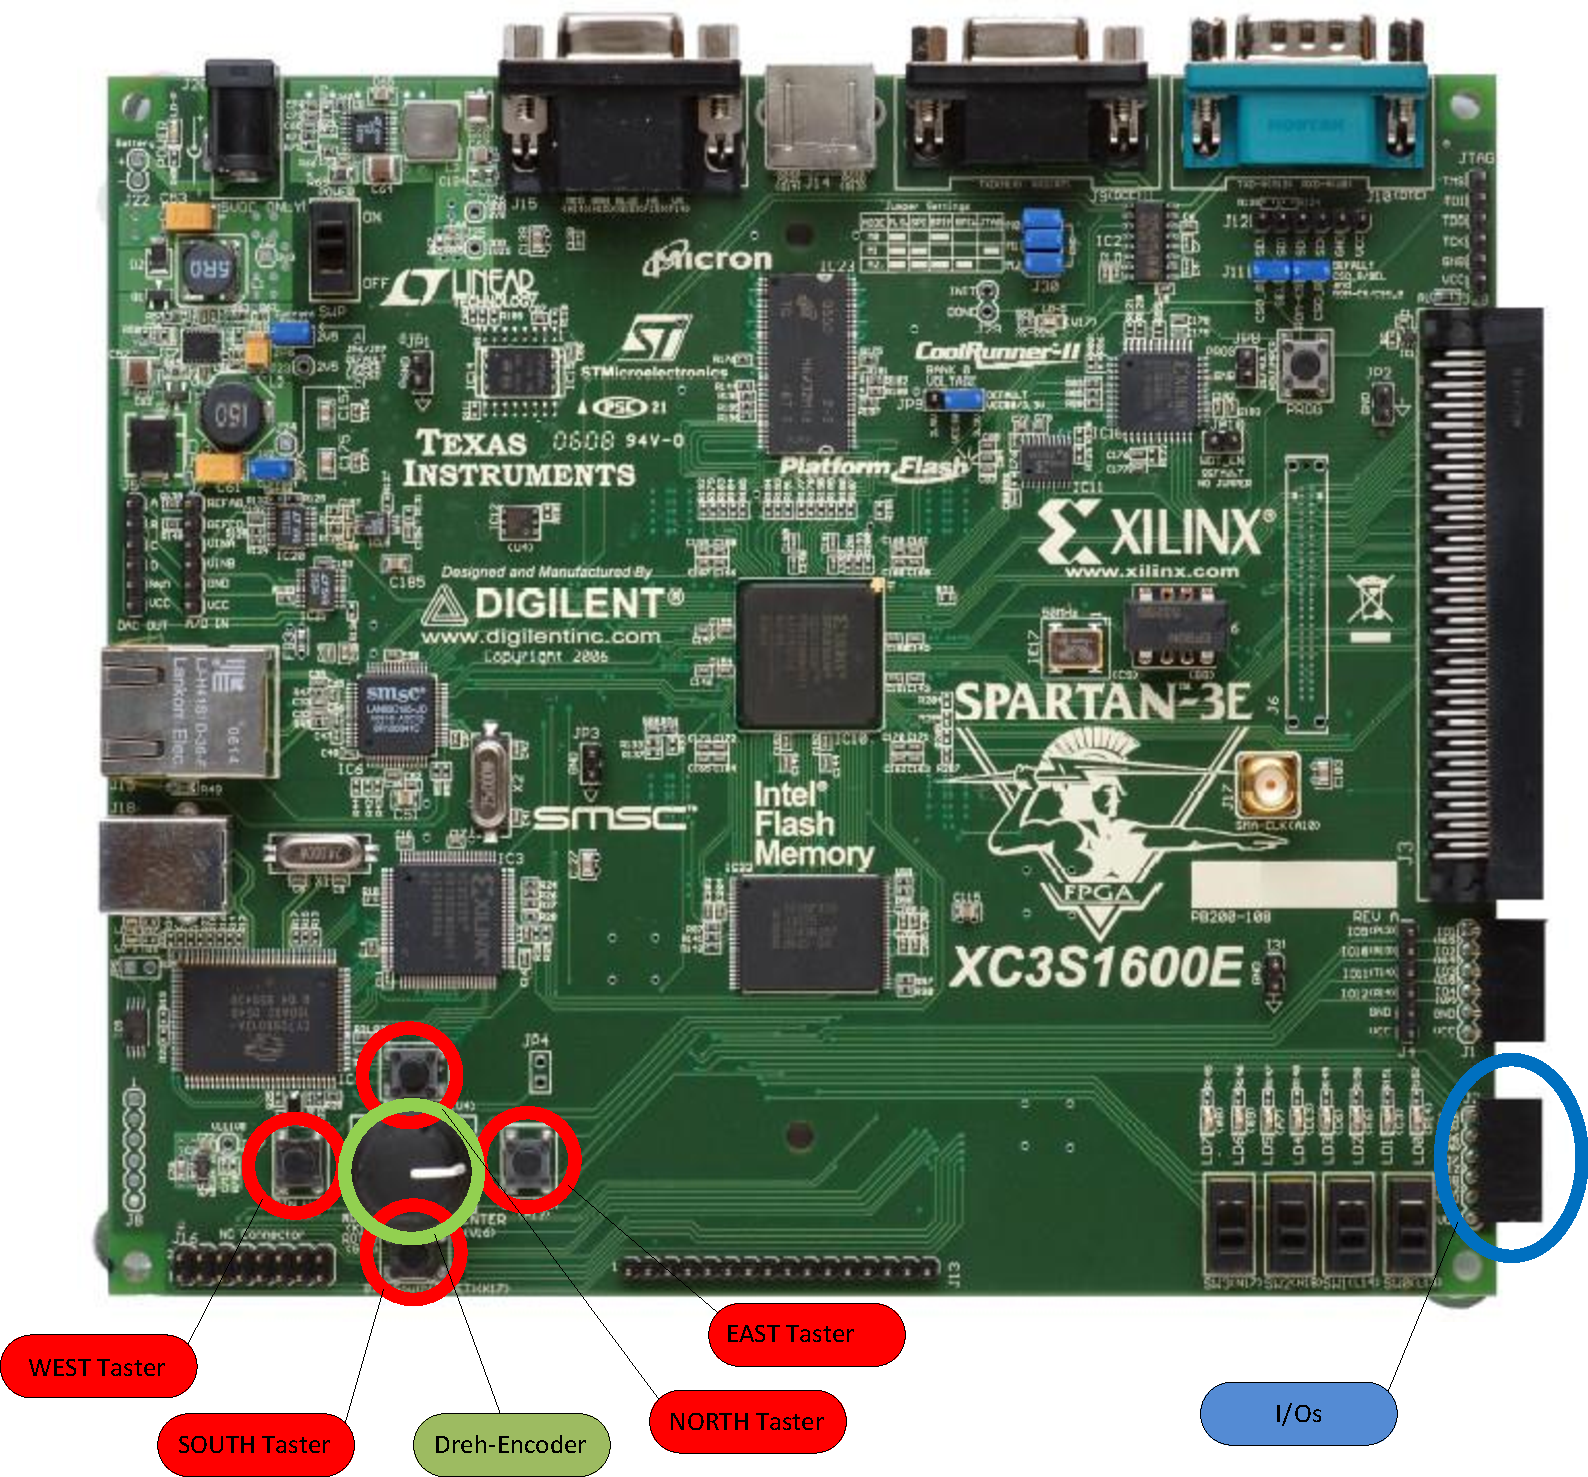
\includegraphics[width=0.70\textwidth]{images/Software-Hardware.pdf}
	\caption{Beschreibung der Ein- und Ausg�nge auf dem Digitalteil}
	\label{fig:Software-Hardware}
\end{figure}

\begin{figure}[ht]
	\centering
		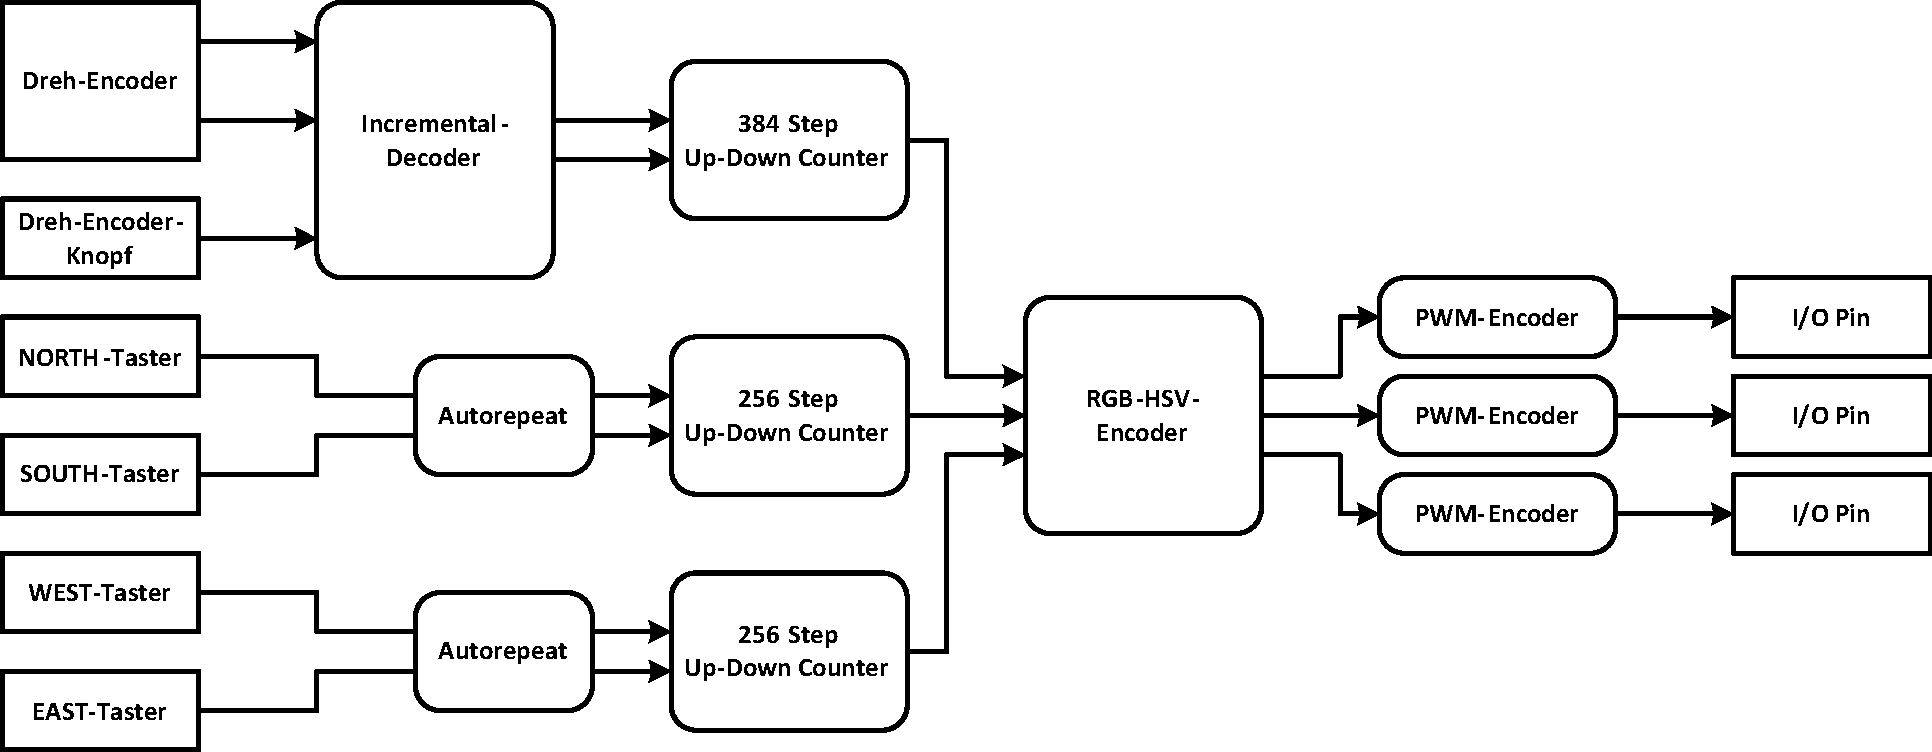
\includegraphics[width=1.00\textwidth]{images/Software.pdf}
	\caption{Blockschaltbild des Digitalteils}
	\label{fig:Software}
\end{figure}


\subsection{HSV-RGB-Encoder}

- basics - bilder von rgb und hsv\\
- bild von den dreiecksfunktionen (trapez) welche die umrechnung visualisieren\\
- erkl�rung, warum beim hue wert nicht 8 bit sondern 9 bit (und 384 schritte) gew�hlt wurden: damit der hue wert auf 6 teil bereiche mit jeweils einer breite mit einer zweierpotenz zerlegbar ist (division durch 64 -> 6 bit nach rechts geschoben)
- system nach fallunterscheidung (6 teilbereiche)

\begin{figure}[ht]
	\centering
		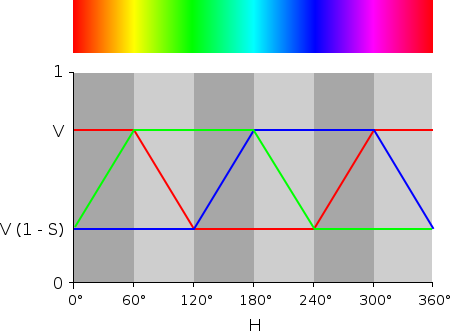
\includegraphics{images/RGB-HSV.png}
	\caption{HSV-RGB Konvertierung}
	\label{fig:RGB-HSV}
\end{figure}


\subsection{Inkremental-Decoder}

- Darstellung der beiden Eingagnssignale (mit sch�n dasrgestelter phasenverschiebung) -> aus spartan pdf\\
- Softeware erkl�rung (evtl. mit state event diagramm)\\
- bild vom drehencoder -> CCW und CW erkl�ren, wieviele steps pro 1 umdrehung -> wieviele umdrehungen f�r ganzer HSV farbraum\\
- Darstellung vom simulator

\begin{figure}[ht]
	\centering
		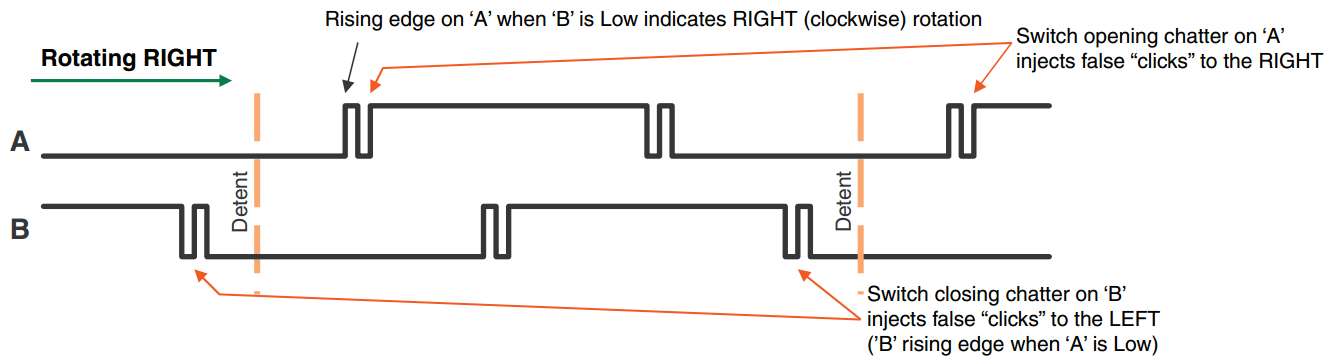
\includegraphics{images/Rotary_signals.png}
	\caption{Ausgangssignale des Dreh-Encoders}
	\label{fig:Rotary_signals}
\end{figure}


\subsection{Up-Down Counter}

- counter erkl�ren\\
- erkl�ren, wieso es 256 und 384 gibt, auch warum der 256 NICHT �berlaufen darf aber der 384 �berlaufen MUSS\\
- Darstellung vom simulator	

\subsection{PWM-Encoder}

- basics eines PWM signals\\
- berechnung der maximalen / minimalen PWM grundtaktfrequenz (argumente: schnell schalten = mehr schaltverluste am FET; langsam schalten = flackern vom auge sichtbar)\\
- basics f�r look-up-table - formel von Mikrocontroller.net: \url{http://www.mikrocontroller.net/articles/LED-Fading}\\
- array in vhdl

\begin{figure}[ht]
	\centering
		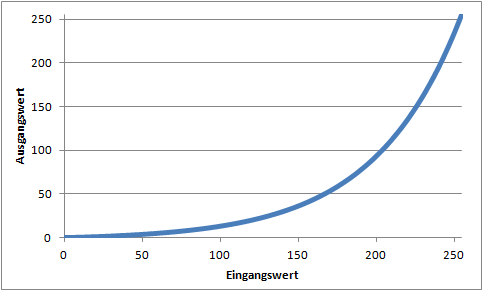
\includegraphics{images/Logarithmiktabelle.png}
	\caption{Logarithmik Umrechnung}
	\label{fig:Logarithmiktabelle}
\end{figure}


\section{Analogteil}
Im analogen Teil des Projekts gings darum, eine high power RGB LED mit einer m�glichst effizienten Schaltung anzusteuern.
\subsection{Bauteilspezifikation}
Bei der Evaluation der LED war die Leistung unser Hauptkriterium. 
\subsubsection{RGB-LED}

\subsubsection{Stromquelle}

\subsection{K�hlk�rperdimensionierung}

\subsection{Hardwareaufbau}

\section{Inbetriebnahme}

\section{Schlussfolgerung}


\vfill
\begin{tabular}{rr}
	\\
	\\
	\\
	\\
	\toprule
	\scriptsize{Datum und Unterschrift}	\hspace{3cm}	&	\textsc{Marcel B�rtschi}	\\
	\\
	\\
	\\
	\\
	\toprule
	\scriptsize{Datum und Unterschrift}	\hspace{3cm}	&	\textsc{Cyril Stoller}
\end{tabular}


% Der Anhang kommt auf eine neue Zeile
\newpage
% Offizielle "A Anhang" Aufz�hlungsvariante
\appendix
% Nur im Inhaltsverzeichnis hinzuf�gen (mit richtiger Seite, da vorher "\newpage"), aber kein Text
\addcontentsline{toc}{section}{Anhang}

% Quellenverzeichnis
%\addcontentsline{toc}{section}{Quellenverzeichnis}
\section{Quellenverzeichnis}
\renewcommand\refname{}

\vspace{-1cm}

\bibliographystyle{amsplain}
\bibliography{Bildquellen}

\end{document}
